\documentclass[12pt]{article}
\usepackage{fullpage,graphicx,psfrag,url}
\usepackage[small,bf]{caption}

\usepackage{amsmath}
\usepackage{amsthm}
\usepackage{amssymb}
\usepackage{verbatim}

\setlength{\captionmargin}{30pt}

\input defs.tex
\newcommand{\sign}{\mathop{\bf sign}}

\bibliographystyle{alpha}

\title{Symbolic Subdifferentiation in Python}
\author{Maurizio Cal\'o and Jaehyun Park\\
EE364B Final Project Progress Report\\
Stanford University, Spring 2010-11}

\begin{document}
\maketitle

\section{Overview}
\subsection{Motivation}
Motivated by the first two weeks of lectures, we decided to create a
Python package (tentative name: Subgradient-PY, or SPY) that solves
optimization problems using subgradient methods. Using SPY, one will
be able to formulate and solve an optimization problem using the
following syntax (subject to change):
\begin{verbatim}
from spy import *
A = rand(20, 5)
x = vector('x', 5)
prob = spy_prob(minimize, norm(x, 1), [A*x <= 1])
prob.solve()
\end{verbatim}

\subsection{Implementation}
Along with CVX-like library functions, SPY will implement three
important classes:
\BIT
\item Expression: Any real-valued mathematical expression is an object
of Expression type. It can contain variables whose values are not
predetermined.
\item Constraint: A constraint is an inequality of the form
$(\text{convex}) \le (\text{concave})$ or an equality of the form
$(\text{affine}) = (\text{affine})$.
\item (Optimization) Problem: A problem is a triplet of the form (minimize/maximize, objective, list of constraints).
\EIT

The essential part of the project is to compute subgradients correctly
and efficiently, since all other methods will rely heavily on subgradients.

\section{Current Progress}
\subsection{Expression Class}
Currently, the expression class only allows scalar-valued expressions.

\subsection{Computation of Subgradients}
The recursive computation of subgradients is based on the composition rule from the class \cite{subg}. Let $f(x) = h(f_1(x), \ldots, f_k(x))$ be a function, where $h$ is nondecreasing convex function, and each $f_i$ is convex. First, we compute the values of $f_1(x), \ldots, f_k(x)$. Then, compute $q \in \partial h(f_1(x), \ldots, f_k(x))$. This results in a vector of length $k$. For each $f_i(x)$, we compute $g_i \in \partial f_i(x)$. Each $g_i$ is a vector of length $k$. Finally, we return the ``weighted sum'' $g$ of the subgradients, namely
\BEAS
g &=& q_1 g_1 + q_2 g_2 + \cdots + q_k g_k \; .
\EEAS

\section{Implementation Details}
\subsection{Forming an Expression}
In the current version of the SPY, one can declare a variable using the following command.
\begin{verbatim}
x = scalar_var('x')
\end{verbatim}
The meaning should be clear from the syntax; the variable whose name is \verb'x' is declared without a value assigned to it.

With variables, it is possible to form a more complicated expression. The following line will create an expression named \verb'ex'.
\begin{verbatim}
ex = expr_sum(expr_abs(expr_sum(x, scalar(-3))), expr_exp(x))
\end{verbatim}
The expression above corresponds to a mathematical expression $|x-3|+e^x$. It should be noted that forming an expression does not immediately compute the value of it. All computations are done lazily; the values will be computed only when the \verb'get_value' method is called on it. Internally, the expression is stored as a tree like the following:

\begin{center}
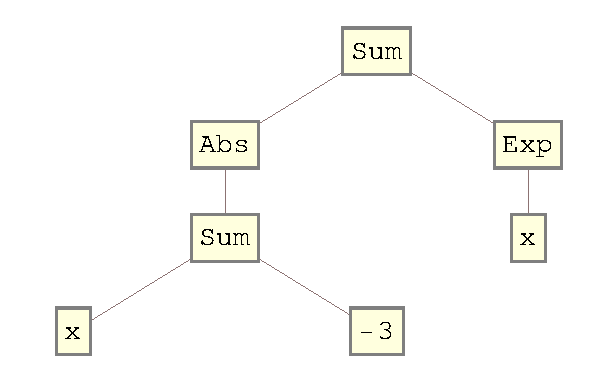
\includegraphics[width=0.5\textwidth]{expr}
\end{center}

\subsection{Retrieving Values or Subgradients}
Because the values of variables in an expression is not predetermined, a user needs to specify them manually in order to retrieve the actual value or a subgradient of the expression. The values of the variables are not passed in as a list of numbers as one might expect. Rather, the values are passed as a dictionary that maps the name of variables to their values.
\begin{verbatim}
varmap = {'x': 0, 'y': 0}
g = ex.subgrad(varmap)
val = ex.get_value(varmap)
\end{verbatim}

\begin{thebibliography}{99}
\bibitem{subg} S. Boyd, \emph{Subgradients}, EE 364B Lecture Slides, 2011.
\end{thebibliography}

\end{document}
